%!TEX TS-program = xelatex
%!TEX encoding = UTF-8 Unicode

\documentclass[11pt, a4paper]{article}

%% Page Layout
\usepackage[margin=2.54cm]{geometry}

\usepackage{enumitem}

\usepackage{euler} % math font package needs to be loaded before others
\usepackage{xunicode,xltxtra, polyglossia}
\setdefaultlanguage[variant=american]{english}

%% fonts, symbols, text
	%%% fonts
	\usepackage{fontspec} %(include if mathspec is not loaded)
	\defaultfontfeatures{Mapping=tex-text, Ligatures=TeX}
	%%% text decoration
	\usepackage[normalem]{ulem} % sout
	%%% semantics symbols
	\usepackage{stmaryrd}
	\usepackage{amsmath,amssymb}
	\newcommand{\transl}{\rightsquigarrow \ensuremath}
	%%% other symbols
	\usepackage{pifont}% http://ctan.org/pkg/pifont
	\newcommand{\cmark}{\ding{51}}%
	\newcommand{\xmark}{\ding{55}}%

%% layout
%%% page layout
\usepackage{multicol}

%% bibliography
	\usepackage[round]{natbib}
	\newcommand{\posscite}[1]{\citeauthor{#1}'s (\citeyear{#1})}
	\renewcommand*{\refname}{\normalsize\textbf{References}\\ \vspace{-.5\baselineskip}}
	\newcommand{\citepos}[1]{\citeauthor{#1}'s \citeyear{\#1}}
	\newcommand{\citeposs}[1]{\citeauthor{#1}'s}
	\newcommand{\citetpos}[1]{\citeauthor{#1}'s (\citeyear{\#1})}

%% figures, examples, diagrams
	%%% examples
	\usepackage{linguex}
	\renewcommand{\firstrefdash}{}
	%%% tables 
	\usepackage{booktabs}
	%%% figures
	\usepackage{graphics}


%% decoration and features
	%%% colors
	\usepackage[dvipsnames]{xcolor}
	\definecolor{orangee}{HTML}{E69F00}
	\definecolor{greenn}{HTML}{009E73}
	\definecolor{bluee}{HTML}{56B4E9}


	%% fonts
	\setmainfont[Scale=MatchLowercase,Mapping=tex-text, SmallCapsFeatures={Letters=SmallCaps}]{Arial}
	\setsansfont[Scale=MatchLowercase,Mapping=tex-text]{Arial}
	\setmonofont[Scale=MatchLowercase]{Andale Mono}

	% spacing
	\parindent=2ex

\begin{document}

\bibliographystyle{plainnat}
\enablehyphenation
% \vspace{-2em}
% \maketitle

\begin{center}
	\textbf{\large%\thetitle
		Projection variability of complement clauses across different operators}
\end{center}

\paragraph{Short summary:} % (fold)
	We examine how the content of embedded complement clauses projects across different entailment-canceling operators for various clause-embedding predicates.
	%
	We measured projection for 20 predicates across four operators: polar questions, negation, modals, and conditionals. Results reveal projection variation by operator and by-predicate variation in the effect of operator on projection.
	%
	Existing theoretical accounts of projection (e.g., \citealt{heim_projection_1983,van_der_sandt_presupposition_1992,abrusan_predicting_2011,schlenker_triggering_2021}) do not capture the observed variability.
	%
	Our findings highlight the importance of considering interactions between predicates and operators and generate important questions for future research on projection.

% paragraph short_summary (end)

\paragraph{Projection across entailment-cancelling operators.}
	Interpreters may infer that a speaker uttering a sentence with an embedded complement clause \ref{ex:family} is committed to the content of the complement (CC, here: \emph{Julian dances salsa,})
	even when embedded under an entailment-canceling operator \Next[a-d]. Then we say that the CC \emph{projects}.

	\ex. \label{ex:family}
		\a. \label{ex:q}
			{\bf Polar Question:} \hfill
			\emph{Did Cole discover that Julian dances salsa?}
		\b. \label{ex:neg}
			{\bf Negation:} \hfill
			\emph{Cole didn't discover that Julian dances salsa.}
		\c. \label{ex:mod}
			{\bf Modal:} \hfill
			\emph{Perhaps Cole discovered that Julian dances salsa.}
		\d. \label{ex:cond}
			{\bf Conditional:} \hfill
			\emph{If Cole discovered that Julian dances salsa, Logan will be joyful.}
		\z.
	\z.
	
	\noindent
	Previous research has investigated projection variability across these operators only rarely, and with conflicting findings.
	%
	For English clause-embedding predicates, \citet{karttunen_observations_1971} proposed a distinction between factives (e.g., \emph{be annoyed, regret}), where the CC projects across all four operators, and semi-factives (e.g., \emph{discover, realize, see, notice}) where it always projects across negation, but not always across the other operators.
	%
	\cite{sieker_projective_2022}, investigating the projection of German clause-embedding predicates across these operators, found an overall pattern of more projection across negation than the others, but no operator/predicate interaction effect.
	%
	%
	In contrast, \citet{smith_relationship_2014} found different projectivity patterns for different types of English projective contents: That of epithets and the CC of \emph{know} were more projective under negation than conditionals, whereas that of non-restrictive relative clauses and \emph{win} showed the opposite pattern.
	%

	Because the studies diverge about whether they find operator/predicate interaction effects, the question arises whether they differ due to cross-linguistic variation, task differences, or different types of contents being tested. To address this, we conducted a series of experiments designed to assess projection across the four entailment-canceling operators in \ref{ex:family}. We used the same projection measure as \citet{sieker_projective_2022} (the `certain that' diagnostic; see e.g., \citealp{tonhauser_how_2018,djarv_prosodic_2017,mahler_social_2020}) and applied it to the CC of 20 English clause-embedding predicates, including factive (\emph{be annoyed, know, reveal}) and semi-factive predicates (\emph{discover, see}),
	and 15 non-factive predicates, given recent findings that their complements may also project, albeit to varying degrees (\citealt{degen_are_2022}).

\paragraph{Method.}
	Projection of the CC of the 20 clause-embedding predicates was measured in four sets of experiments: Predicates were embedded in polar questions in Exps.\ 1, under negation (Exps.\ 2), under a modal {\em perhaps} (Exps.\ 3), and in conditional antecedents (Exps.\ 4). (Each set contained three experiments using different at-issueness measures in a separate block. Here, we focus on the projection ratings.)
	%
	Participants read utterances like in \ref{ex:family} and rated whether the speaker (who was named) was certain of the CC (e.g.: \emph{\lq Is [the speaker] certain that Julian dances salsa?\rq}), on a slider marked \emph{`no'} (coded as \texttt{0}) at one end and \emph{`yes'} (coded as \texttt{1}) on the other. Each participant saw all 20 clause-embedding predicates (each with a unique content from a set of 20) under one operator. We analyze data from $2,682$ self-reported native speakers of American English, recruited on Prolific or Amazon's MT platform.


\begin{figure}[ht]
	\vspace{-.5\baselineskip}
	\centering
	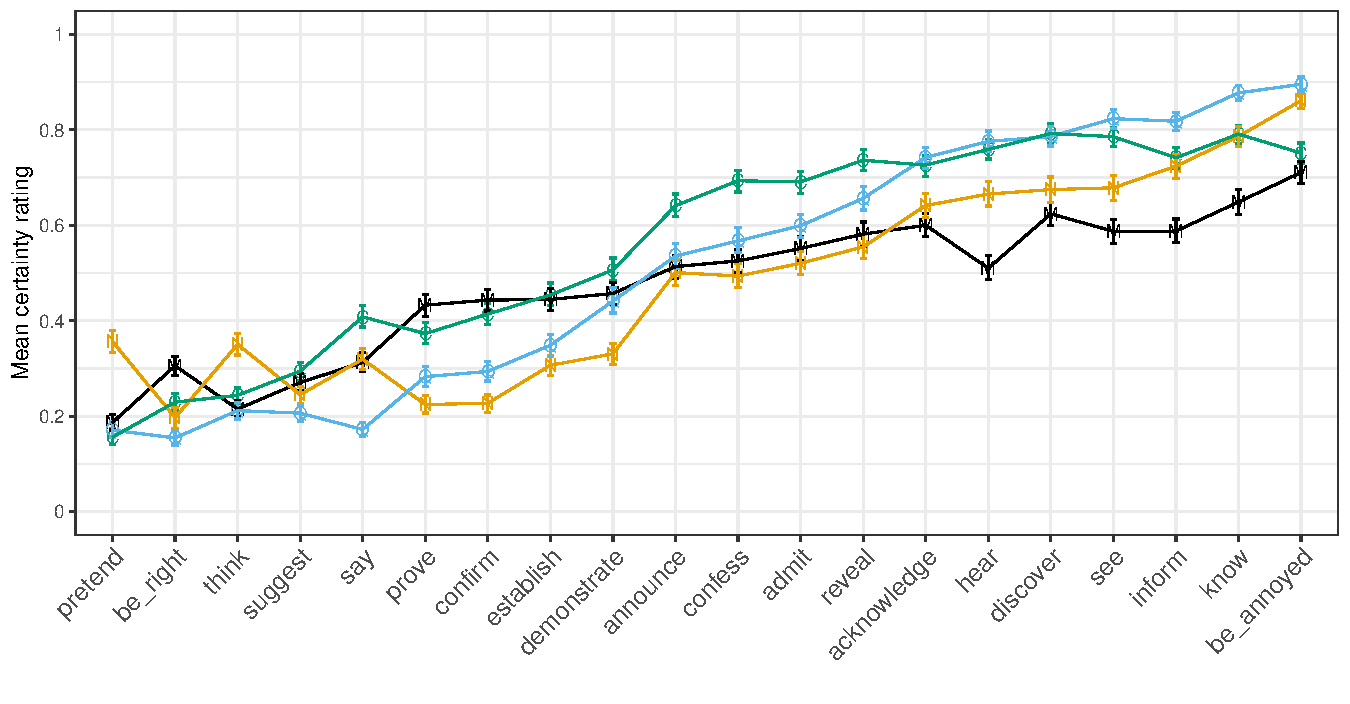
\includegraphics[width=\textwidth]{graphs/proj-by-both.pdf}
	\caption{\small Mean certainty ratings by predicate and operator with 95\% bootstrapped confidence intervals. Entailment-cancelling operator coded by letter and color:  \textcolor{orangee}{\texttt{N}: negation}, \texttt{M}: modals, \textcolor{greenn}{\texttt{C}: conditional antecedents}, \textcolor{bluee}{\texttt{Q}: polar questions}.}
	\label{fig:figure1}
\end{figure}

\paragraph{Results and Analysis.}
	Our analysis reveals two key results: \textbf{(i)} There is projection variability by operator, with higher mean projection ratings for question-operators (Maximum likelihood estimate: $0.51$) than negation (MLE: $0.48$) and modals ($0.47$), but lower than for conditional antecedents ($0.56$, see model \#1 in Table\ \ref{t:models}).
	%
	This differs from \posscite{sieker_projective_2022} observation that the CC of German clause-embedding predicates projects more across negation than the other operators, suggesting potential cross-linguistic variation in the projection of clausal complements across entailment-canceling operators.
	
	\textbf{(ii)} There is by-predicate variation in the effect of operator on projection, as illustrated in Figure~\ref{fig:figure1}, showing mean projection ratings for the 20 clause-embedding predicates by operator, with predicates ordered by their mean rating across operators (\emph{be annoyed} has the highest overall mean).
	%
	For instance, the CC of \emph{be annoyed} projects more across negation and questions than conditionals and modals, and the CC of \emph{discover} projects less across negation than conditionals and questions, but more across negation than modals. The CC of \emph{know} projects less across negation than questions, but more across negation than modals, while the difference between negation and conditionals is not significant.
	%
	These generalizations are supported by models\ \# 2--4 in Table\ \ref{t:models}, which also each have at least $34$ highly significant interaction terms (out of $57$ possible interactions of operator and predicate).
	%

	Our finding of operator/predicate-interactions concurs with \citet{smith_projection_2011}, but we did not reproduce their result that the CC of \emph{know} projects more from negation than conditionals.
	%
	Further, our finding differs from the result of \citet{sieker_projective_2022}, who found no interaction between predicates and operators. Given that the methods and the set of projective contents of our experiment were very similar to theirs, this may suggest cross-linguistic variation in projection variability (cf. \citealt{tonhauser_projection_2020}).
	%
	Additionally, our results are contradict \posscite{karttunen_observations_1971} distinction between factive and semi-factive predicates: The CC of (factive) \emph{be annoyed} does not project invariably across four operators, and the CC of \emph{discover,}  considered semi-factive, does not project more from under negation than the other three operators. The pattern observed for {\em know} does not fit into either category.
	
% paragraph results (end)
	
\paragraph{Discussion.}
	Our results---that various entailment-canceling operators affect projection differently and that there is by-predicate variation in the effect of operator on projection---are not captured by contemporary projection analyses, for several reasons.
	%
	First, they do not predict variation associated with different types of entailment-cancelling operators. In \citet{heim_projection_1983}, for instance, the CC of (semi-)factive predicates projects to the global context, except when that would produce an inconsistency and the CC is accommodated locally. While it is conceivable for operator meanings to systematically affect the possibility of local accommodation, this has not been spelled out.
	%
	The second reason is that many analyses only focus on (semi-)factive predicates, whose CCs are analyzed as presuppositions (e.g., \citealt{heim_projection_1983,van_der_sandt_presupposition_1992}), or entailed CCs that project unless at-issue with respect to the Question Under Discussion (e.g., \citealt{abrusan_predicting_2011,simons_best_2017}). This limits their predictive power for other predicates.
	%
	\posscite{schlenker_triggering_2021} may be an exception, which predicts the potential of projection for CCs that are contextually entailed. In the full paper, we discuss how Schlenker's analysis may be extended to capture the gradient projection observed in our experiment.
	%
	Finally, no current analysis makes sufficiently fine-grained distinctions between different clause-embedding predicates (but only between whether the CC is presupposed/entailed or not). Consequently, precluding predictions about the by-predicate variation in operator effects.

	Our results further question \posscite{karttunen_observations_1971} proposed distinction between factive and semi-factive predicates (see also \citealt{beaver_have_2010,sieker_projective_2022}).
	Future research appealing to these categories must clarify their definition. 
	% Additionally, claims about projection variability must be relativized to the entailment-canceling operator.
	% Although our data replicate the result from \citet{tonhauser_how_2018} that, in polar questions, the CC of \emph{discover} is less projective than that of \emph{know}, the same does not hold in conditionals.
	%
	Finally, our results provide further support (from negation, modals, and conditionals) for the result of \citet{degen_are_2022}, that projection does not categorically differentiate between (semi-)factive and non-factive predicates: The CCs of \emph{\lq inform\rq} and \emph{\lq acknowledge\rq}, for instance, are at least as projective as those of some (semi-)factive predicates.
	%
	% Further, the variability we found is gradient, confirming previous research that by-predicate variability is not determined by categorical lexical classes (\citealt{tonhauser_how_2018,degen_are_2022}),
	% and extending this result to by-predicate variability in interaction with entailment-cancelling contexts.
	%
	In a full presentation, we would discuss how more fine-grained lexical distinctions may affect projection variability: For example, the CCs of \emph{\lq think\rq} and \emph{\lq pretend\rq} (which are often used anti-veridically) project more across negation than other operators. The CCs of \emph{\lq reveal, confess, admit\rq} and \emph{\lq announce\rq} (communicative achievement predicates) project most from conditional antecendents.
	
% \noindent
% {\bf Discussion: Novel research question.}

	% So, can the observed interaction between predicate and operator in mean projection ratings be predicted from lexical semantic/pragmatic properties of the predicates, and, if so, how?
	% This is a pressing question for future research, to which our data offer some tentative answers. We identify four major patterns.
	% %
	% The predicates \emph{pretend} and \emph{think} exhibit the {\bf `Negation high'} pattern, shown in panel (a) of \textbf{Figure~2}: We tentatively hypothesize that negation (but not the other operators) interacts with the semantic or pragmatic antiveridicality associated with these predicates.
	% %
	% The inferential predicates \emph{prove, confirm}, and \emph{establish} exhibit a {\bf `Negation low'} pattern, shown in panel (b): Here, we tentatively hypothesize that the veridical meaning component interacts with negation (but not the other operators), to result in lower projection ratings under negation.
	% %
	% For \emph{announce, confess, admit}, and \emph{reveal}, the CC is most projective when embedded in conditional antecedents: This {\bf `Conditional high'} pattern (c) may suggest that the discourse effect of a conditional interacts with the change-of-state communication predicates.
	% %
	% Finally, the predicates  \emph{inform, know}, and \emph{be annoyed} exhibit a {\bf `Modal low'} pattern (d). The lexical meaning of these predicates, whose CCs are among the most projective, appears to interact with the modal adverb {\em perhaps}, yielding lower projection ratings.

	%%%%%
	% In spite of a lack of categorical distinctions about the projection behavior of our verbs, we can find some interesting patterns. \textbf{Fig.~\ref{fig:figure2}} gives the mean certainty ratings for the four operators by predicate, identifying some groups of predicates that show similar by-operator variation. We highlight four \lq projection-profiles\rq here: \emph{pretend} and \emph{think} are the only predicates that are most projective under negation compared to all other operators (\texttt{N} $>$ \texttt{M, Q, C}). \emph{annouce, confess, admit,} and \emph{reveal} are most projective under conditionals, while there is also a tendency that there is more projection from questions compared to modals and negation, a difference that may not be robust for \emph{announce} (\texttt{C} $>$ \texttt{Q} \textcolor{gray!40}{$>_?$} \texttt{M, N}). \emph{prove, confirm,} and \emph{establish} are more projective under modals and conditionals than under questions and negation (\texttt{M, C} $>$ \texttt{Q, N}). Finally, \emph{inform} and \emph{know} are most projective under questions, and least projective under modals (\texttt{Q} $>$ \texttt{N, Q} $>$ \texttt{M}).




\begin{table}[h]
	\centering
	\begin{tabular}{llrrrr}
		Model & & Estimate & Std. Error & t-value\\
		\midrule
		\#1 & Intercept: \emph{question} & 0.51 & 0.01 & 44.78 & ***\\
		& operator: conditional & 0.05 & 0.01 & 5.30 & ***\\
		& operator: modal & -0.04 & 0.01 & -4.45 & ***\\
		& operator: negation & -0.03 & 0.01 & -4.67 & ***\\
		\midrule
		\#2 & Intercept: \emph{\bf be annoyed}/negation & 0.87 & 0.01 & 79.86 & ***\\
		& operator: conditional & -0.12 & 0.02  & -7.36 & ***\\
		& operator: modal & -0.16 & 0.02  & -10.01 & ***\\
		& operator: question & 0.02 & 0.01 & 1.72 & n.s.\\
		\midrule
		\#3 & Intercept: \emph{\bf discover}/negation & 0.68 & 0.01 & 62.70 & ***\\
		& operator: conditional & 0.11 & 0.02 & 7.11 & ***\\
		& operator: modal & -0.06 & 0.02 & -3.63 & ***\\
		& operator: question & 0.10 & 0.01 & 7.08 & ***\\
		\midrule
		\#4 & Intercept: \emph{\bf know}/negation & 0.79 & 0.01 & 72.97 & ***\\
		& operator: conditional & 0.00 & 0.02 & -0.06 & n.s.\\
		& operator: modal & -0.14 & 0.02 & -9.18 & ***\\
		& operator: question & 0.08 & 0.01 & 5.67 & ***\\
		\bottomrule
	\end{tabular}
	\caption{\small Excerpt of the output from three linear mixed effects models; \textbf{\#1} has fixed effects of operator; random effects: participant and item intercepts, \textbf{\#2-4} have fixed effect: operator, predicate, and their interaction; random effect: participant intercepts.
		Models were fit with \texttt{lme4, lmertest} in \texttt{R}. Models \textbf{\#2--4} also had at least $34$ highly significant interaction terms of \texttt{operator} and \texttt{predicate} with $p < 0.001$ (not shown here).}\label{t:models}
\end{table}

% \hspace{-2.7em}
% 	\begin{minipage}{\textwidth}\centering
% 	\begin{tabular}{p{.5\linewidth} p{.5\linewidth}}
% 		\parbox{\linewidth}{\centering (a) \textbf{Negation high}\\
% 		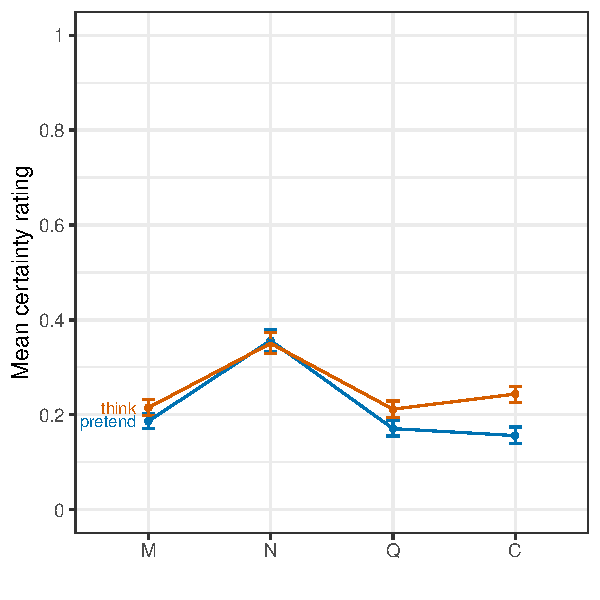
\includegraphics[width=.8\linewidth]{graphs/profile1.pdf}}
% 		&
% 		\parbox{\linewidth}{\centering (b) \textbf{Negation low}\\
% 		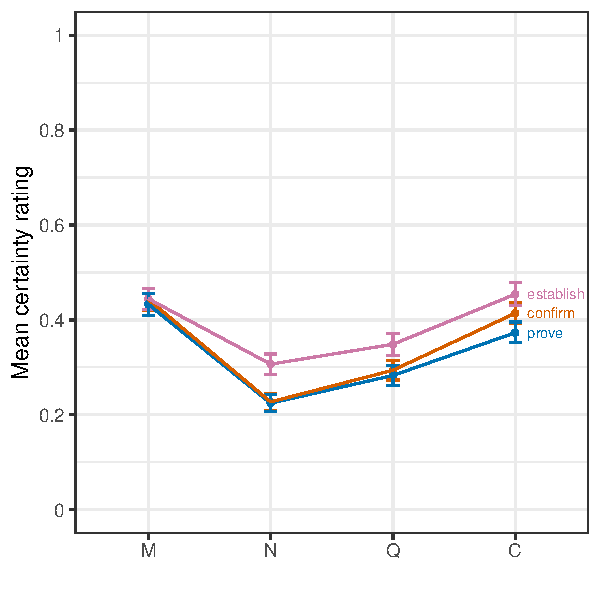
\includegraphics[width=.8\linewidth]{graphs/profile4.pdf}}
% 		\\
% 		\parbox{\linewidth}{\centering (c) \textbf{Conditional high}\\
% 		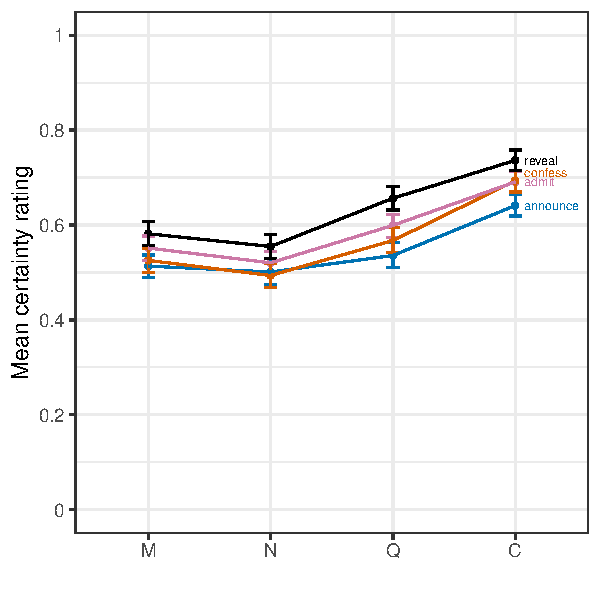
\includegraphics[width=.8\linewidth]{graphs/profile2.pdf}}
% 		&
% 		\parbox{\linewidth}{\centering (d) \textbf{Modal low}\\
% 		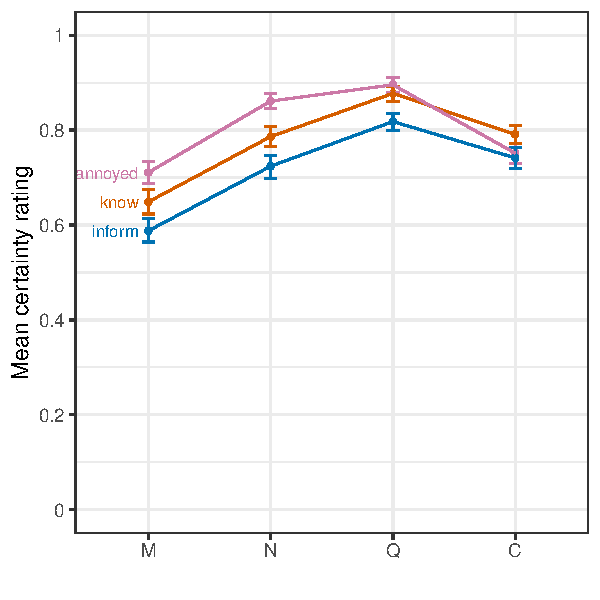
\includegraphics[width=.8\linewidth]{graphs/profile5.pdf}}
% 		\\
% 	\end{tabular}
% \end{minipage}

% \vspace{-.4\baselineskip}
% \noindent \small Figure 2: \small Mean certainty ratings by operator (\texttt{M}: Modal, \texttt{N}: Negation, \texttt{Q}: Polar Question, \texttt{C}: Conditional antecedent) with 95\% bootstrapped confidence intervals, for some groups of predicates (\lq predicate patterns\rq).

% \begin{figure}[h]
% 	\hspace{-2.5em}
	
% 	\vspace{-\baselineskip}
% 	% \caption{Mean certainty-ratings by operator for four predicate patterns in our data.}
% 	\label{fig:figure2}
% \end{figure}

\newpage

% \bibliography{../bibliography.bib}
\bibliography{../projective-content.bib}

\end{document}